%; whizzy chapter
% -initex iniptex -latex platex -format platex -bibtex jbibtex -fmt fmt
% 以上 whizzytex を使用する場合の設定。


%     Tokyo Debian Meeting resources
%     Copyright (C) 2008 Junichi Uekawa

%     This program is free software; you can redistribute it and/or modify
%     it under the terms of the GNU General Public License as published by
%     the Free Software Foundation; either version 2 of the License, or
%     (at your option) any later version.

%     This program is distributed in the hope that it will be useful,
%     but WITHOUT ANY WARRANTY; without even the implied warranty of
%     MERCHANTABILITY or FITNESS FOR A PARTICULAR PURPOSE.  See the
%     GNU General Public License for more details.

%     You should have received a copy of the GNU General Public License
%     along with this program; if not, write to the Free Software
%     Foundation, Inc., 51 Franklin St, Fifth Floor, Boston, MA  02110-1301 USA

%  preview (shell-command (concat "evince " (replace-regexp-in-string "tex$" "pdf"(buffer-file-name)) "&"))
% 画像ファイルを処理するためにはebbを利用してboundingboxを作成。
%(shell-command "cd image200812; ebb *.png")

%%ここからヘッダ開始。

\documentclass[mingoth,a4paper]{jsarticle}
\usepackage{monthlyreport}

% 日付を定義する、毎月変わります。
\newcommand{\debmtgyear}{2008}
\newcommand{\debmtgmonth}{12}
\newcommand{\debmtgdate}{20}
\newcommand{\debmtgnumber}{47}

\begin{document}

\begin{titlepage}
\thispagestyle{empty}

% タイトルページ:編集必要な部分は最初のマクロに飛ばすこと

\vspace*{-2cm}
第\debmtgnumber{}回 東京エリア Debian 勉強会資料

\hspace*{-2.4cm}
\includegraphics[width=210mm]{image200801/2008title.eps}\\
\hfill{}\debmtgyear{}年\debmtgmonth{}月\debmtgdate{}日

\end{titlepage}

\dancersection{Introduction}{上川 純一}
 
 今月のDebian勉強会へようこそ。これからDebianの世界にあしを踏み入れると
 いう方も、すでにどっぷりとつかっているという方も、月に一回Debianについ
 て語りませんか?

 Debian勉強会の目的は下記です。

\begin{itemize}
 \item \underline{Debian Developer} (開発者)の育成。
 \item 日本語での「\underline{開発に関する情報}」を整理してまとめ、アップデートする。
 \item \underline{場}の提供。
 \begin{itemize}
  \item 普段ばらばらな場所にいる人々が face-to-face で出会える場を提供
	する。
  \item Debian のためになることを語る場を提供する。
  \item Debianについて語る場を提供する。
 \end{itemize}
\end{itemize}		

 Debianの勉強会ということで究極的には参加者全員がDebian Packageをがりがり
 と作るスーパーハッカーになった姿を妄想しています。情報の共有・活用を通し
 て Debianの今後の能動的な展開への土台として、「場」としての空間を提供す
 るのが目的です。

以上を目的とした、2008 年アジェンダです:
\begin{enumerate}
 \item 新年会「気合を入れる」
 \item Open Source Conference Tokyo (3/1)
 \item データだけのパッケージを作成してみる、
       ライセンスの考え方 (David Smith)
 \item バイナリ一つのパッケージを作成してみる (吉田@板橋)\\
       バージョン管理ツールを使いDebianパッケージを管理する(git)\\
       アップストリームの扱い(svn/git/cvs)(岩松 信洋さん)
 \item バイナリの分けたパッケージの作成。(前田さん)\\
       バイナリの分け方の考え方、アップグレードなどの運用とか。
 \item パッケージ作成(dpatch/debhelperで作成するパッケージ)(小林儀匡さん)\\
       man の書き方(roff or docbook)(でんさん)
 \item パッケージ作成(kernel patch、kernel module)
       、Debconf発表練習
 \item Debconf アルゼンチン、共有ライブラリパッケージ作成

 \item Open Source Conference Tokyo/Fall、
       デーモン系のパッケージの作成、\LaTeX{}、 emacs-lisp、フォントパッケージ
 \item パッケージの cross-compile の方法、amd64 上で i386 のパッケージと
       か、OSC-Fall報告会、Debconf報告会
 \item 国際化 po-debconf / po化 / DDTP
 \item 忘年会
\end{enumerate}


\newpage

\begin{minipage}[b]{0.2\hsize}
 \definecolor{titleback}{gray}{0.9}
 \colorbox{titleback}{\rotatebox{90}{\fontsize{80}{80} {\gt デビアン勉強会} }}
\end{minipage}
\begin{minipage}[b]{0.8\hsize}
\hrule
\vspace{2mm}
\hrule
\tableofcontents
\vspace{2mm}
\hrule
\end{minipage}

\dancersection{事前課題}{上川 純一}

今回の事前課題は以下のうちどれかです:

\begin{enumerate}
 \item Debian勉強会で今年やったこと、来年したいこと
 \item \LaTeX{}+Gitの事前課題ができなかった、こんなハマり方しました体験記
\end{enumerate}

この課題に対して提出いただいた内容は以下です。

%; whizzy-master ../debianmeetingresume200812-presentation.tex
%%; whizzy-master ../debianmeetingresume200812.tex

\begin{prework}{������}

��ǯ��ä���ǯ��ꤿ�����Ȥ�ͤ��Ƥߤޤ�����

\preworksection{��ǯ��ä�����}

\begin{itemize}
 \item ��ǯ�κǽ�˷ײ�򤿤ƤƤߤ����ǽ�Ū�ˤϤ��Τޤ޼»ܤϤ��ʤ��ä�
       ���ɡ��ʤ�餫�Υ����ǥ��θ����ˤϤʤä���
 \item \LaTeX{} �Υϥ󥺥�����ä���
 \item Debian �ѥå����������Τ���ΰ�Ϣ�ιֺ¤��äƤߤơ�
       �������ֻ���򤤤������ʿͤ����ˤ��Ƥ��ä���
\end{itemize}
�Ȥ����Τ�����ޤ�����

\preworksection{��ǯ��ꤿ���ʤ��ȻפäƤ���Τ�}

���������ȥϥ󥺥���Ū�ʤ�Τ����䤷�Ƥ���������

\begin{itemize}
 \item DocBook�Υϥ󥺥���
 \item �ѥå����������Υϥ󥺥���
 \item avahi �γ��ѹֺ�
 \item \LaTeX{}��Ϣ�Τ������ΥХ���ľ����
 \item screencast / �ӥǥ�����ե���� / ���ȥ꡼�ߥ󥰴�Ϣ�β���
\end{itemize}
�������ͤ��Ƥ��ޤ���

\end{prework}

\begin{prework}{ʿ߷�ӷ�}

\preworksection{Debian�ٶ����ǯ��ä����ȡ���ǯ����������}
�����3���λ��äǤ���
�ǥӥ���⤽���Ǥ���������ʤ����Ȥ��餱�ʤΤǡ�
��ǯ�ϳ��оޤ�ͤ餤�Ĥġ������ȤǤ���褦�ˤʤ�Ȥ����ʤ�

\preworksection{\LaTeX{}+Git�λ������꤬�Ǥ��ʤ��ä�������ʥϥޤ������ޤ����θ�
       ��}
\LaTeX{}�Ϥޤ������Ĥ����ʤ�Ƥ������ʤΤǥ��ȥ쥹̵�Ǥ�����
�ӥ�vi�ʤ錄���ˤ�emacs���ʤ�Ȥ⤤�������Ϥ�����
�äƤ��󤸤ǤȤƤ��ϫ���Ƥ��ޤ���
���������ʸ�Ϥ������Τ�10ʬ���餤�����äƤ����Ǥ���

���������β�����̤��Ƥޤ��褯�狼�äƤ��ʤ��ʤ���
������Ȥ�����
\begin{itemize}
 \item git������
 \item ����ޥ����ʤ��Ȥ���santaku�Ȥ�)
 \item �����Ƥ����ޤä���
\end{itemize}

����ʤ�ΤǴ��ۤ��Ƥ�������

\end{prework}
\begin{prework}{ƣ������}

\preworksection{��Debian�ٶ���Ǻ�ǯ��ä����ȡ���ǯ���������ȡ�}

��ǯ�ϡ�3��ޤǤϴ���Debian�ٶ���4����������ꥢDebian�ٶ���˻���
���ޤ����ʲ��٤��������塼����Թ�ǻ��äǤ��ޤ���Ǥ������ˡ�
����ܿ������μ��˿������Ȥ������ǡ��ٶ���Ȥ�����ϼ�ʬ�ˤȤä�̥��
Ū�ʤ�ΤǤ��������٤Ƥ���٤˵ۼ�����Τ��񤷤����Ȥ�ƨ������Τ⤢���
���������������λ���������뤳�Ȥ����꤬�����Ǥ���

��Ū�˺�ǯ��ȿ�ʤȤ��ơ�
\begin{itemize}
\item �ٶ���ǰ���줿���Ƥ��Ф��ơ���ʬ��try and error�λ��֤���ݤǤ�
      �ʤ��ä�
\item �ٶ����Debian Project���Ф��Ʋ���׸����Ƥ��ʤ�
\end{itemize}
�Ȥ���2������ǯ�ϲ������Ƥ��������ȹͤ��Ƥ��ޤ���

\preworksection{��ǯ��}

�嵭��Ƨ�ޤ��� \textbf{��1�桼�������æ�ѡ�}���ܻؤ��ƴ�ĥ����
�Ȼפ��ޤ������Τ���ˤޤ���
\url{http://www.debian.or.jp/community/devel/}�˽񤤤Ƥ��뤳�Ȥ�ǯ��ǯ��
�����Ѥ������򤷤Ƥ��������Ȼפ�����Ǥ���

\end{prework}
\begin{prework}{���Ĺ�ʿ}
\preworksection{Debian �ٶ���Ǻ�ǯ��ä����ȡ�}

��ǯ�ϡ��ѥå������κ�����ȯɽ��Ԥ��ޤ������������ä����ĥå��ߤ򤤤���
��ĺ�����Τˡ������������Ƥ��ʤ��ä����Ȥ������Ȥ˺����ʤ��鵤�Ť��ޤ�
������������Ǥ��͡�
���Ȥϡ�Debian �� ``��''�Ͻв񤤷Ϥ�``��''�˹׸��������ȡ��ʤ��

\preworksection{��ǯ�ؤη��ɽ����}
\begin{itemize}
 \item �ͥ���ȯɽ���ٶ���α��Ĥˤ�ä��Ѷ�Ū�˻��褷�Ƥ����ޤ�������ʤ��ơ�\textbf{``����
��''}��
 \item Debian �ٶ���ؤλ��üԡ�Debian �γ�ȯ�Ԥ����䤹�������ˡ��ͤ�
       �ޤ���
 \item ���� Debian �桼���ˤ��ơ��ٶ����Ϣ��Ƥ��ޤ���
\end{itemize}

\end{prework}
\begin{prework}{���Ĥ���}

\preworksection{��Debian�ٶ���Ǻ�ǯ��ä����ȡ�}

�ٶ���˻��ä��ơ�

\begin{itemize}
 \item �ѥå�����������Ϣ(OSC�ǤΥϥ󥺥���ޤ�)
 \item \LaTeX{}�ϥ󥺥���
\end{itemize}
���ٶ��ˤʤä���
�ʤ�Ȥʤ��ѥå����������Ǥ���褦�ˤʤäƤ����Τǡ��⤦���ʥ��ƥåץ��å�
��������

\preworksection{��Debian�ٶ������ǯ���������ȡ�}

��ɸ�Ȥ��Ƥϡ�
\begin{itemize}
 \item �ٶ���λ��ò�������䤹
 \item �����η����ٶ���Debian Project�˹׸�������
\end{itemize}

�ٶ���Υͥ��Ȥ��Ƥϡ�
\begin{itemize}
 \item �ѥå���������
 \item �Х���ݡ��ȥϥ󥺥���
 \item �絬�ϤʴĶ��ǤΡ�Debian�����д�����ˡ���ѥå������ΰ���Ŭ�ѤȤ�
       ����ե�����δ����Ȥ����ºݱ��Ѥ��Ƥ��������ä�ʹ���Ƥߤ����Ǥ���
\end{itemize}
�Ȥ��ä������Ǥ��礦����

\end{prework}
\begin{prework}{��ޤ�������}

\textbf{Debian�ٶ���Ǻ�ǯ��ä����ȡ���ǯ����������}

�ٶ���ˤ�11��黲�ä��Ϥ᤿�Ф���� Debian �鿴�ԤʤΤǡ���ǯ��ä����Ȥ�
��ǰ�ʤ����Ĥ����ʤ��ΤǤ���...

\textbf{��ǯ��ä�����}

\begin{itemize}
\item avahi �ν����λؼ�����Ȥ��Ƥ����Τǡ������� DHCP server ����
      �����������ˤ���ޤ���(Windows �� VMware ��� Debian ��ư�����Ƥ�������)
\item \TeX ��������
\end{itemize}

\preworksection{��ǯ����������}

\begin{itemize}
 \item git �Υϥ󥺥���
 \item �ѥå����������Υϥ󥺥���
 \item �����Υϥ󥺥���
\end{itemize}
�����꤬�Ǥ���Ȥ����ʤ��ȻפäƤ��ޤ���

\end{prework}
\begin{prework}{���� ʸ}
\begin{itemize}
\item Debian�ٶ���Ǻ�ǯ��ä�����\\
��ǯ���ؤ���ٶ���ϻ��ä��ޤ���Ǥ�����������
�Ȥꤢ���������DD�ϻ��ߤޤ�����

\item  ��ǯ����������\\
����Ū�ʻ��Ǥ���,��ä�C��kernel���ٶ�������Ǥ���
���server��Tuning���äȽ����褦�ˤʤꤿ����
����Ȼ��������οͤ�õ�����������ǥޥޤǥ����ƥ��äƤ���ͤ��ʤ����ʤ�������

 \item \LaTeX{}+Git�Ǥ���ʥϥޤ������ޤ����θ���\\
anthy+scim�����Ϥ����ƤʤΤǤ��ʤ���֤�������ޤ�����
\end{itemize}

\end{prework}
\begin{prework}{���� ����}

\preworksection{Debian�ٶ���Ǻ�ǯ��ä�����}
��ǯ�ϡ�debhelper+CDBS+quilt/dpatch�ǤΥѥå������󥰤˴ؤ����äȡ�
Po4a���Ѥ����������ƥʥ󥹤ˤĤ��Ƥ��ä򤷤ޤ�����

\preworksection{Debian�ٶ������ǯ����������}
��ǯ�ϡ�buildd���Ѥ�����ư�ӥ�ɤˤĤ����ä��Ǥ�����Ȼפ��ޤ���
�ޤ�������äȼ��ư�����ƤߤƤ��뤳�Ȥ������Ĥ�����Τǡ�
������⤦����������Ȥ����������ˤ���ȯɽ�������Ǥ���

�Ǹ�ˡ���ǯ������Debian Developer�ˤʤꤿ���Ǥ���

\end{prework}
\begin{prework}{�����ϥ�}
\begin{itemize}
\item Debian�ٶ���Ǻ�ǯ��ä�����\\
���פ������פϷ򹯾����ͳ�ǡ����ޤ껲�äǤ��ޤ���Ǥ����ͤ���
���פǤϡ���ǯstable���ѼԤˤ⤫����餺sid��Ƴ�������ꡢ
��ǯ�֤��TeX�����ä��ꡢ�����Ÿ���ˤʤäƤ��ޤ����ʺ��⡦������

\item  ��ǯ����������\\
�ٶ���λ������꤬������ʹߤ⤳�η����ˤʤ�ʤ�С�emacs��Ф��ʤ���
�����ʤ��Τ��ʤ���������Ū��*nix�Ķ��Ǥϡ�vi�ɤʤΤǤ�����
�ʡ������ȸ�����ꡢemacs�ޤä����Ȥ��ޤ��󡪡�
\end{itemize}

\end{prework}
\begin{prework}{���ܡ���Ƿ}
��ǯ�⤢�ޤ��礷�����Ȥ�ʤ����˲᤮��äƤ��ޤ��ޤ�����

\textbf{��ǯ��ä�����}
\begin{itemize}
\item �Ρ��侾���󤬹ֱ餷�� live-helper �λȤ������������OSC �ˤ� Live
      DVD �����ۤ��ޤ�����
\item ���Ӥ���ιֱ�˿�ȯ���졢CDBS �ˤƥѥå���������ޤ�����
\end{itemize}

\textbf{��ǯ����������}
\begin{itemize}
\item �Ѹ���ٶ����������ط� (���ɤȤ�) �Ǥ�׸���������
\item emacs ���äȤ��ޤ��Ȥ���褦�ˤʤꤿ���Ǥ� (��)
\end{itemize}

\end{prework}
\begin{prework}{�侾 ����}
\preworksection{��ǯ}

��ǯ�ϰʲ��Τ褦�ʤ��Ȥ�Ԥ��ޤ�����
\begin{itemize}
 \item Debian�ѥå������󥰥ϥ󥺥�����ä���
 \item Git �ˤɤäפ�ȤĤ��ä���
 \item git-buildpackage / VCS �� Debian�ѥå������ˤĤ��ƹͤ��Ƥߤ���
 \item �����ͥ�¦����Υѥå������˴ؤ��륢�ץ������򤷤Ƥߤ���\\
   Linux kernel patch / kernel module �ˤĤ����ä�����
 \item ��ɤ��ä���
 \item Ustream ��Ȥä����ȥ꡼�ߥ󥰤�Ԥä���
 \item ����������ؤ�ĩ��(Perl/Ruby/Lua)��������ؤλ��ä�Ԥä���
 \item ¾���ٶ���ȤΥ���ܤ򤷤���
 \item �ٶ��񱿱Ĥ�Ԥä���
 \item ���ݡ��Ȥ���ѥå����������䤷����
\end{itemize}

\preworksection{��ǯ����ɸ}

\begin{itemize}
 \item DD�ˤʤ�
 \item SH �ݡ��ƥ��󥰡�wanna-build/buuildd �ط�
 \item ��̥쥤������Ȥθ�ή
 \item �ӥǥ��ط������ȥ꡼�ߥ󥰤Υ��ݡ��ȶ���
 \item �����ͥ�ط��Ǥ� Debian�ؤι׸�
\end{itemize}

\end{prework}


\dancersection{最近のDebian関連のミーティング報告}{上川 純一}
\subsection{東京エリアDebian勉強会46回目報告}
% (query-replace-regexp "<.*?>" "")
% (query-replace-regexp "^[	 ]\+" "")

東京エリアDebian勉強会報告。
2008年11月15日土曜日に11月の第46回東京エリアDebian勉強会を実施しました。
今回の参加者は
青木さん、平澤さん、明渡さん、やまだたくまさん、
前田耕平さん、伊藤弘和さん、山本浩之さん、
濱野司さん、でん@相模原さん、じつかたさん、
森田尚さん、岩松さん、kenichiro matohara さん、
小林さん、北原さん、鈴木崇文さん、藤沢理聡さん、
吉田@板橋さん、日比野啓さん、やまねひできさん、上川x2の22名でした。

今回は私にとっての初のハンズオンイベントの進行役です。感想を
つらつらと書いてみます。

最初に会場のネットワークの設定を行いました。有線ネットワー
クを必要とする人が多く、無線以上に設定が時間がかかりました。
また、avahi (autoipd) でネットワークを構築するという手法を
理解していない参加者が大半で、dhcp が無いため設定できないと
いうコメントをいただきました。無線で、avahi で接続するとい
う方針は野心的すぎたかもしれませんね。会場の電源容量がたり
るかどうかひやひやしましたが、ブレーカーはおちなかったよう
です。最初の30分を費やしましたが、Git 演習の部分を省略すれ
ばすむので、諦めました。ネットワーク関連のその他の問題とし
て Git サーバが安定して稼働しない、Debian Mirror が動かない
という問題がありました。とりあえず、はらはらどきどきです。


開始後数十分以上遅刻してきた人が数人居ましたが基本的にはサ
ポートする余裕はありませんでした。今ネットワークの設定なん
てしなくてよいから!


事前に準備していた項目は一通り説明しました。参加者がうまく
操作できていたかどうかは講師をしていた側としてはよくわかり
ません。


宴会で聞いたところハンズオンをしたのでよくわかったというコ
メントも、途中で理解できないところがあったというコメントも
ありました。次回以降もハンズオン形式を継続してみるべきなの
かどうかは判断に迷います。


漢字入力ができないというのは、sid をインストールするだけで
何も漢字入力方法を設定してこないとは想定していなかったので、
課題には記述していませんでした。

漢字が表示できないというのは
\debianbug{506165}が根本原因だっ
たようです。
当日は原因がよく分からなかったため、リカバリできませんでした。
今後は\debianbug{506047}などと合わせて改善していくでしょう。


\subsection{Debian Meeting With Coffee}

2008年12月3日に Debian Meeting With Coffee が開催されました。
参加者はやまねひできさん、山本浩之さん、いわまつさん、本庄さん、小笠原徳
彦さん、ボール
デアンドレアスさん、藤沢理聡さん、はしもとまささん、でんすけさん、吉田@板橋
さん、id774.netさん、ssig33さん、やまださん、yuisekiさん、mizunoさん、い
ちいたかしさん、たかはしさん、じつかたさん、日比野啓さん、KenichiroMATOHARAさん、し
まだ M. ひろふみさん、平澤さん、みやはらとおるさん、まえだでした。\footnote{参加していたのに載っていない、あるいは参加できなかったのに載っている方
がいらっしゃいましたらお詫びします。}

まず、みやはらさん、場所とコーヒーをご提供下さり、ありがとうございました。コー
ヒーごちそうさまでした。


今回の趣旨は、『よりカジュアルな形で Debian についての諸々の話の場を設け
(中略)、コーヒーでも飲みつつ Debianについて気軽に言葉を交わしてみません
か?』ということでした。ですので、コーヒーを飲みながらゆるい感じでのんび
りと Debian についての雑談をしながら過ごす
ものとばかり思っていました。
ところが、開始1時間後頃にのんびりやってきたところ、
すでに参加者による三番目のネタ発表が行われていました。皆さん一応コーヒーは手元にお
いてすすっているものの、``カジュアル''とはとてもかけ離れた熱い説明と質
問が飛び交っていました。趣旨を間違えたわけではないんですよね。きっとみん
な、Debian について語りたくて語りたくて仕方なかったのですね。
お初の参加者が結構多かったのは、いつもの Debian 勉強会はたまたま都合が合わなくて
参加できなかったのに違いありません。今まで Debian 勉強会に参加されたこと
がない方も、今回の DMC をきっかけに、今後は継続的に Debian 勉強会に参加して
くれるに違いありません。


ネタ発表は当日参加された方だけの特典としておくとして\footnote{単に覚えて
いないだけとも言う。}、今後の勉強会のネタだし討論会が岩松さん主導で行わ
れました。そこで決まったものは以下のとおりです。
\begin{itemize}
 \item N 台のサーバ管理方法
 \item プレゼン環境
 \item IPv6 の話
 \item Debian 勉強会 LT をやりたい。LT のやり方、練習。LT を考える
 \item AtomPCでDebian →工人舎マシンやeeePCでの導入レポート(橋本さん)
 \item updateしたいときにどうするのか →その展開方法について
 \item パケットフィルタリングの設定が楽な ipfw, natd を Debian で使えるよ
       うにしてみる。(本庄さん)
 \item Web 系の開発
 \item 組み込み関係の話 →インストーラのデバッグの話(前田)
 \item Ubuntu → Debian 移行方法どれが良いのか? ベストな移行の検討
 \item Window Manager を熱く語る
 \item Debian で NAS (日比野さん)
 \item ドライバオートビルド (岩松さん)
 \item Debian デバッグ方法 →開発環境
 \item 他のディストロの人を呼ぶ
 \item VM の話
 \item ZFS on Debian をフルスクラッチ(でんさん)\footnote{ご自身の誕生
       日までに。}
 \item YaST on Debian を使えるようにし、SUSE から乗り換える。
\end{itemize}

名前が挙がっている人、そうでない人、それぞれですが、来年も Debian はネタ
の宝庫ですね。




\dancersection{各種イベント開催実績}{上川 純一}
\label{sec:debmtg2008results}
\index{debianjp@Debian JP} 
\index{とうきょうえりあ@東京エリアDebian勉強会}

Debian 開発者の育成を目的として開催してきた東京エリアDebian勉強会も今回
で4年目が終了しました。
事前課題事後課題を設定しており、予習復習を必要だとうたっている勉強会です
が、実際にどれくらい実施されているのか、まずは事前課題の実施実績を確認し
てみましょう。
\fgref{fig:attendandprepostwork}です。
各月の数字は\tbref{tab:attendandprepostwork}です。

% sqlite> .separator ' & ' 
% sqlite>  select year, month, sum(type='attendance'), sum(type='prework'), sum(type='postwork') from attend group by year,month order by year, month ;

\begin{figure}[ht]
 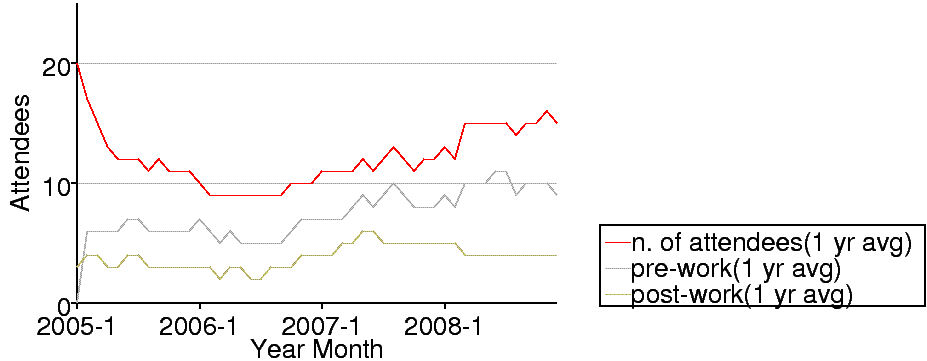
\includegraphics[width=1\hsize]{image200812/memberanalysis/attend.png}
\caption{東京エリアDebian勉強会事前課題・事後課題提出実績(12ヶ月移動平均)}\label{fig:attendandprepostwork}
\end{figure}

\begin{table}[ht]
 \caption{東京エリアDebian勉強会事前課題・事後課題提出実績}\label{tab:attendandprepostwork}
\begin{minipage}{0.5\hsize}
\begin{tabular}{|l|r|r|r|r|}
 \hline
   年&月 & 参加人数 & 事前課題 & 事後課題 \\
 \hline
 2005 & 1 & 20 & 0 & 3 \\
 2005 & 2 & 15 & 12 & 6 \\
 2005 & 3 & 10 & 8 & 4 \\
 2005 & 4 & 9 & 6 & 2 \\
 2005 & 5 & 6 & 6 & 4\\
 2005 & 6 & 13 & 10 & 5\\
 2005 & 7 & 12 & 7 & 4\\
 2005 & 8 & 9 & 6 & 2\\
 2005 & 9 & 14 & 7 & 4\\
 2005 & 10 & 10 & 5 & 3\\
 2005 & 11 & 7 & 6 & 3\\
 2005 & 12 & 8 & 5 & 3\\
 2006 & 1 & 9 & 7 & 3\\
 2006 & 2 & 8 & 4 & 2\\
 2006 & 3 & 6 & 0 & 0\\
 2006 & 4 & 15 & 11 & 6\\
 2006 & 5 & 7 & 2 & 1\\
 2006 & 6 & 14 & 9 & 4\\
 2006 & 7 & 2 & 2 & 4\\
 2006 & 8 & 17 & 9 & 7\\
 2006 & 9 & 12 & 8 & 5\\
 2006 & 10 & 22 & 15 & 7\\
 2006 & 11 & 3 & 12 & 7\\
 2006 & 12 & 15 & 7 & 4\\
\end{tabular}
\end{minipage}
\begin{minipage}{0.5\hsize}
\begin{tabular}{|l|r|r|r|r|}
 \hline
   年&月 & 参加人数 & 事前課題 & 事後課題 \\
 \hline
 2007 & 1 & 15 & 6 & 4\\
 2007 & 2 & 13 & 8 & 4\\
 2007 & 3 & 0 & 6 & 16\\
 2007 & 4 & 18 & 14 & 6\\
 2007 & 5 & 21 & 14 & 7\\
 2007 & 6 & 1 & 0 & 1\\
 2007 & 7 & 18 & 12 & 3\\
 2007 & 8 & 25 & 18 & 5\\
 2007 & 9 & 0 & 7 & 5\\
 2007 & 10 & 10 & 1 & 6\\
 2007 & 11 & 19 & 10 & 6\\
 2007 & 12 & 11 & 11 & 4\\
 2008 & 1 & 22 & 11 & 4\\
 2008 & 2 & 0 & 1 & 0\\
 2008 & 3 & 37 & 27 & 11\\
 2008 & 4 & 17 & 13 & 3\\
 2008 & 5 & 20 & 14 & 3\\
 2008 & 6 & 10 & 8 & 2\\
 2008 & 7 & 17 & 12 & 4\\
 2008 & 8 & 10 & 0 & 4\\
 2008 & 9 & 17 & 13 & 5\\
 2008 & 10 & 11 & 0 & 7\\
 2008 & 11 & 22 & 14 & 6\\
\end{tabular}
\end{minipage}

\end{table}

昨年からは勉強会は東京と関西の両方で開催されるようになっています。
東京エリアDebian勉強会と、関西Debian勉強会について簡単に出席数で実績をみてみましょう。
まず、東京についてグラフにしてみると\fgref{fig:peoplechart}になります。

\begin{figure}[h]
 \begin{center}
  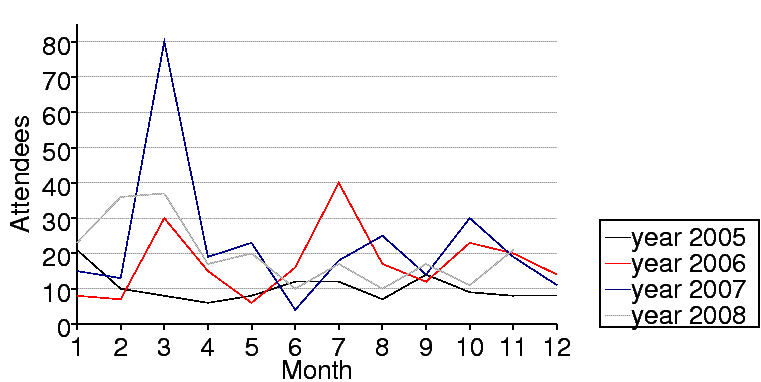
\includegraphics[width=1\hsize]{image200812/people-chart.png}
  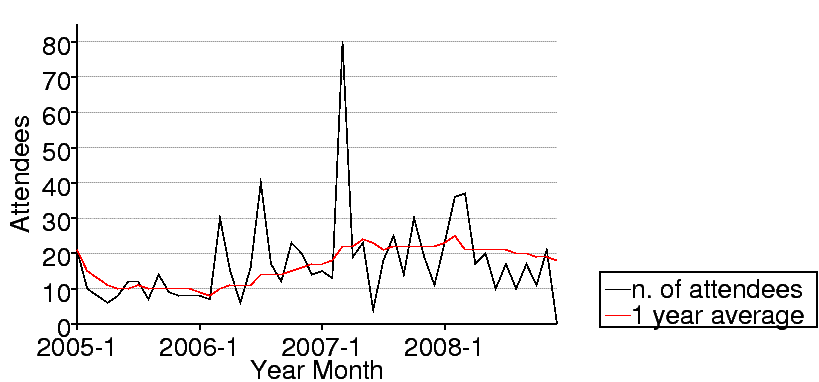
\includegraphics[width=1\hsize]{image200812/serialized.png}
 \end{center}
\caption{東京エリアDebian勉強会の参加人数推移}
\label{fig:peoplechart}
\end{figure}


具体的な数字と、トピックを見てみましょう。
 
\begin{table}[ht]
\begin{minipage}{0.5\hsize}
 \caption{東京エリアDebian勉強会参加人数(2005年)}\label{tab:count}
 \begin{center}
  \begin{tabular}{|l|c|p{10em}|}
 \hline
   & 人数 & 内容 \\
 \hline
   2005年1月 & 21 & 秘密\\
   2005年2月 & 10 & debhelper1\\
   2005年3月 & 8 &  (早朝) debhelper2、social contract\\
   2005年4月 & 6 & debhelper3\\
   2005年5月 & 8 & DFSG、dpkg-cross、lintian/linda\\
   2005年6月 & 12 & alternatives、d-i\\
   2005年7月 & 12 & toolchain、dpatch\\
   2005年8月 & 7 & Debconf参加報告、ITPからアップロードまで\\
   2005年9月 & 14 & debconf\\
   2005年10月 & 9 & apt-listbugs、バグレポート、debconf翻訳、debbugs\\
   2005年11月 & 8 & DWN翻訳フロー、statoverride\\
   2005年12月 & 8 & 忘年会\\
 \hline
  \end{tabular}
 \end{center}
\end{minipage}
\begin{minipage}{0.5\hsize}
 \caption{東京エリアDebian勉強会参加人数(2006年)}\label{tab:count2006}
 \begin{center}
  \begin{tabular}{|l|c|p{10em}|}
 \hline
 & 参加人数 & 内容\\
 \hline
 2006年1月 & 8 & policy、Debian勉強会でやりたいこと\\
 2006年2月 & 7 & policy、multimedia \\
 2006年3月 & 30 & OSC: debian勉強会、sid \\
 2006年4月 & 15 & policy、\LaTeX{} \\
 2006年5月 & 6 & mexico \\
 2006年6月 & 16 & debconf、cowdancer\\
 2006年7月 & 40 & OSC-Do: MacBook Debian \\
 2006年8月 & 17 & 13執念 \\
 2006年9月 & 12 & 翻訳、Debian-specific、oprofile \\
 2006年10月 & 23 & network、i18n会議、Flash、apt \\
 2006年11月 & 20 & 関西開催: bug、sid、packaging \\
 2006年12月 & 14 & 忘年会 \\
 \hline
  \end{tabular}
 \end{center}
\end{minipage}
 \end{table}

\begin{table}[t]
\begin{minipage}{0.5\hsize}
 \caption{東京エリアDebian勉強会参加人数(2007年)}\label{tab:count2007}
 \begin{center}
  \begin{tabular}{|l|c|p{10em}|}
 \hline
 & 参加人数 & 内容\\
 \hline
2007年1月 & 15 & 一年を企画する \\
2007年2月 & 13 & dbs, dpatch\\ 
2007年3月 & 80 & OSC仮想化 \\
2007年4月 & 19 & quilt, darcs, git\\
2007年5月 & 23 & etch, pbuilder, superh \\   
2007年6月 & 4 & エジンバラ開催:Debconf7 実況中継 \\
2007年7月 & 18 & Debconf7 参加報告\\
2007年8月 & 25 & cdn.debian.or.jp \\   
2007年9月 & 14 & exim \\   
2007年10月 & 30 & OSC Tokyo/Fall(CUPS) \\   
2007年11月 & 19 & live-helper, tomoyo linux kernel patch, server\\
2007年12月 & 11 & 忘年会\\
 \hline
  \end{tabular}
 \end{center}
\end{minipage}
\begin{minipage}{0.5\hsize}
 \caption{東京エリアDebian勉強会参加人数(2008年)}\label{tab:count2008}
 \begin{center}
  \begin{tabular}{|l|c|p{10em}|}
 \hline
 & 参加人数 & 内容\\
 \hline
2008年1月 & 23 & 一年を企画する \\
2008年2月29+1日 & 36 & OSC  \\
2008年3月 & 37 & データだけのパッケージ、ライセンス \\
2008年4月 & 17 & バイナリパッケージ \\
2008年5月 & 20 & 複数のバイナリパッケージ \\
2008年6月 & 10 & debhelper \\
2008年7月 & 17 & Linux kernel patch / module パッケージ \\
2008年8月 & 10 & Debconf IRC会議とDebian温泉 \\
2008年9月 & 17 & po4a, 「Debian メンテナのお仕事」 \\
2008年10月 & 11? & OSC Tokyo/Fall \\
2008年11月 & 17 & 「その場で勉強会資料を作成しちゃえ」 Debian を使った \LaTeX{} 原稿作成合宿 \\
2008年12月 & ? & 忘年会 \\
 \hline
  \end{tabular}
 \end{center}
\end{minipage}
\end{table}

それでは、関西Debian勉強会の出席状況を確認してみましょう。
グラフで見ると\fgref{fig:kansaipeoplechart}になります。
表で見ると\tbref{tab:count2007kansai}

\begin{figure}[h]
 \begin{center}
  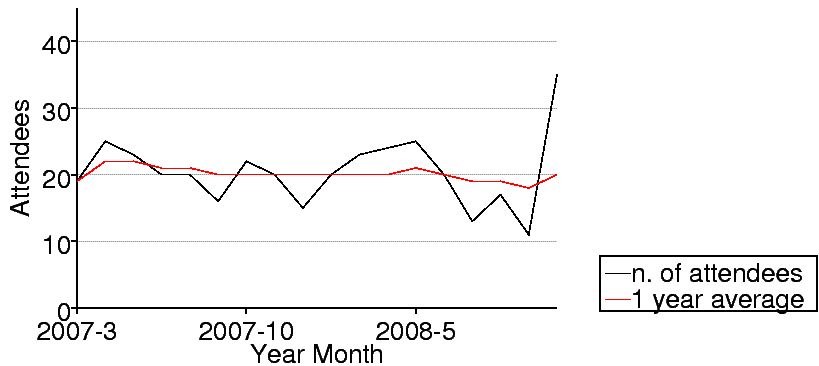
\includegraphics[width=1\hsize]{image200812/kansai.png}
 \end{center}
\caption{関西の参加人数推移}
\label{fig:kansaipeoplechart}
\end{figure}


\begin{table}
\begin{minipage}{0.5\hsize}
 \caption{関西Debian勉強会参加人数(2007年)}\label{tab:count2007kansai}
 \begin{center}
  \begin{tabular}{|l|c|p{10em}|}
 \hline
 & 参加人数 & 内容 \\
 \hline
2007年3月 & 19 & 開催にあたり \\
2007年4月 & 25 & goodbye、youtube、プロジェクトトラッカー\\
2007年6月 & 23 & 社会契約、テーマ、debian/rules、bugreport\\
2007年7月 & 20前後 & OSC-Kansai \\
2007年8月 & 20 & Inkscape、patch、dpatch\\
2007年9月 & 16 & ライブラリ、翻訳、debtorrent\\
2007年10月 & 22& 日本語入力、SPAMフィルタ\\
2007年11月 & 20前後 & KOF \\   
2007年12月 & 15& 忘年会、iPod touch\\   
 \hline
  \end{tabular}
 \end{center}
\end{minipage}
\begin{minipage}{0.5\hsize}
 \caption{関西Debian勉強会参加人数(2008年)}\label{tab:count2008kansai}
 \begin{center}
  \begin{tabular}{|l|c|p{10em}|}
 \hline
 & 参加人数 & 内容 \\
 \hline
2008年2月 & 20 & PC Cluster, GIS, \TeX \\
2008年3月 & 23 & bug report, developer corner, GPG \\
2008年4月 & 24 & coLinux, Debian GNU/kFreeBSD, sid \\
2008年5月 & 25  & ipv6, emacs, ustream.tv\\
2008年6月 & 20  & pbuilder, hotplug, ssl\\
2008年8月 & 13  & coLinux \\
2008年9月 & 17  & debian mentors, ubiquity, DFSG\\
2008年10月 & 11  & cdbs,cdn.debian.or.jp \\
2008年11月 & 35  & KOF \\
2008年12月 & ?  & \\
 \hline
  \end{tabular}
 \end{center}
\end{minipage}
\end{table}

\dancersection{2008年を振り返ってみる}{上川 純一}

\subsection{最近のトレンドと今後の推移}

最近どんなことが
あって、これからどういうことがあるでしょうか。
みんなで予想してみましょう。

{\footnotesize
\begin{tabular}[t]{|p{8em}|p{8em}|p{12em}|p{8em}|p{8em}|}
\hline
2006 &2007 &2008 &2009 & 2010 \\
\hline
%2006
IntelMacに、coreduoでdual-core CPU に、 

glantank(ARM)、 
OpenMicroServer(MIPS)、 

OpenSolarisが出てDebian/Solaris (Nexenta) 登場、 
SparcT1がオープンに、

CC3.0、

Qwik登場(?)、

雑誌が大多数消失、

 &
%2007
VT・AMD-V(仮想化技術)が普及(ML115!)、

黒箱(ARM)、
OpenBlocks(PPC?)、
iPhone登場、 
HSDPA 月額5000円くらいに、
google mobile、

VISTAリリース、 
Leopardリリース、 

GPL3.0、
メモリ2Gがコモディティーに、
SparcT2がオープン、 
ニコニコ動画、
& 
%2008
python 3.0
ruby 1.9

wine 1.0, wine64 登場

RoR 2.0 登場で普及に

4コア・64bit のCPUがデスクトップに普及、
Core2Quad 値下げ。

ニコニコ動画1000万ユーザ突破、
初音ミクブームに

地デジ関連のPC製品の普及

勉強会の普及(楽天とか)

公衆無線LAN (wireless gate)

携帯電話の売上が落ちる、
iPhone, Android 登場、
emobile 100円PC抱きあわせ
(eeePC, Dell mini9)
Zaurus販売終了。

Chumby 発売。

サーバの仮想化 ESXi・シンクライアント

MacBook Air 発売、
無線 802.11n が実機に

SystemZ10 発表

世界経済の崩壊(IT投資緊縮財政、職を失う人が増加)

FreeBSD 7 (malloc, ZFS ?)

Debian次世代育成計画始動

Debian Maintainer 制度始動

セキュリティー関連(OpenSSL 事件、DNS事件)

クラウド関連が流行?

Nintendo DSi

&
%2009

tile window manager boom ?

Lenny リリース予定

Debian 合同結婚式

デスクトップ、8コア、4GB? 8GB?

ノートパソコン、2コア、2GB?

Linux が標準インストールのPC。

SSD の値段と容量がこなれる?
HDDがなくなる?高くなる?

ファイルシステムかわる?

ipv6 使えるようになってる?

Bluray が普及?

DL禁止法? torrent に逆風?

&
%2010

消費税上昇に伴う繁忙期

クラウドにより、単純なホスティング業者がつづかない?
一部は自社でもつようになる?

Squeezeリリース

USB 3.0 搭載、wireless USB vs Bluetooth ?

組み込みCPUはAtomに統一?Armは残ってる?

kFreeBSD オフィシャルアーキテクチャに

ruby 2.0 リリース?

 \\

\hline
\end{tabular}

}

\subsection{SWOT}

%SWOT
{\large
\begin{tabular}[t]{|p{8em}|p{8em}|p{8em}|p{8em}|}
\hline
できたこと & できなかったこと & チャンスとなるもの & 脅
 威となるもの \\
\hline
%S 
嫁ができた。(20\%、10\% 2次元)
将来のDDが生まれた。

Hands-on(パッケージ作成と\LaTeX{}) と合宿(温泉とブレスト)、
DMCができた。

持ち回りで発表する

場所がいろいろだった。(上川不在)

他の勉強会(カーネル読書会)に殴り込み(岩松、山根)

Ubuntuとの交流、Debian JPに寄付



&
%W

当初の目標であった女子高生、大学生への勧誘が成功しなかった。

嫁ができなかった(70\%、想像力がたりない)

発表やりたかったけどできなかった(でんさん)

GNU/Hurd、SuperH

Debconfにいけなかった(上川以外)

日本へのDebconf招致活動未完

&
%O
	 
所帯持ちハック方法が生まれる(いかにして時間をつくるか)。

無駄な買い物をしなくなる。
ハックしないと。

東京オリンピックの成立?

学生の就職率低下、大学院生増加?ニート増加?

GPLv3 の普及?
Android?

&
%T

環境整備ができなくなる(
ボーナスが減った、
仕事がなくなるかも)

Atom によるCPUアーキテクチャーの駆逐

ハックできないデバイスの増加(電話とか)

法制度の強化により自由がうばわれる?

従量制課金に移行?

\\
\hline
\end{tabular}
}

\subsection{SWOT 2}

% SWOT 2
{\large
\begin{tabular}[t]{|p{4em}|p{11em}|p{11em}|p{11em}|}
\hline
 &  & チャンスとなるもの & 脅威となるもの  \\\hline
\vspace{0.2\vsize}~

 & & 
%O
	 
所帯持ちハック方法が生まれる(いかにして時間をつくるか)。

無駄な買い物をしなくなる。
ハックしないと。

東京オリンピックの成立?

学生の就職率低下、大学院生増加?ニート増加?

GPLv3 の普及?
Android?

&
%T

環境整備ができなくなる(
ボーナスが減った、
仕事がなくなるかも)

Atom によるCPUアーキテクチャーの駆逐

ハックできないデバイスの増加(電話とか)

法制度の強化により自由がうばわれる?

従量制課金に移行?

\\
\hline
できたこと & 
%S

嫁ができた。(20\%、10\% 2次元)
将来のDDが生まれた。

Hands-on(パッケージ作成と\LaTeX{}) と合宿(温泉とブレスト)、
DMCができた。

持ち回りで発表する

場所がいろいろだった。(上川不在)

他の勉強会(カーネル読書会)に殴り込み(岩松、山根)

Ubuntuとの交流、Debian JPに寄付

&

東京オリンピックの会場でハック。

学校にお願いして学生を勧誘する・ハンズオン。

「君のさわっているXXはLinuxだけどより詳しく知りませんか?」
(ミニノートのプリインストール、携帯、Android)

& 

よりよいネットワークプロトコルを実施

アンチAtom?

\\
\hline

できなかったこと
&
%W

当初の目標であった女子高生、大学生への勧誘が成功しなかった。

嫁ができなかった(70\%、想像力がたりない)

発表やりたかったけどできなかった(でんさん)

GNU/Hurd、SuperH

Debconfにいけなかった(上川以外)

日本へのDebconf招致活動未完

&

Debconf にいく。

時間をつくる、ライフハック(所帯持ちハック)。

専門学校、工業高校、大学での開催。


言語系のコミュニティーに切り込む

インフラ系の人たちに切り込む

非常勤講師になる。

&

\\
\hline
\end{tabular}
}


\dancersection{sqlite3 と python で csv ファイルを分析する}{上川純一}
\label{sqlite3intro}
\index{sqlite}

sqlite はお手軽に SQL を利用するための仕組みです。データベースが一つの
UNIXファイルとして管理されており、データベースの作成・削除が簡便に行うこ
とができること、また、サーバクライアントアーキテクチャではなく、OSの提供
するファイルシステムのロック機構を活用してACID特性を実現しているという特
徴があります
(\fgref{fig:sqlitestructure})\footnote{\url{http://www.sqlite.org/atomiccommit.html}
に仕組みの説明があります}。
データベースを利用する場合においては、データベースをサーバクライアントモデルで利用しよう
とすると、
データベースファイル置き場やポート番号やホスト名や
ユーザ名やパスワードの設定が最低でも必要になりますが、それらが必要なくな
ります。
そのため、データベースのインスタンスを別に立ち上げなくてもよいんだけど、
ちょっと SQL を使いたいというようなクイックハックに便利です。

\begin{figure}[ht]
\begin{center}
 \fbox{\includegraphics[width=0.5\hsize]{image200812/sqlite.eps}}
\end{center}
\caption{一般的なDBと sqliteの違い}\label{fig:sqlitestructure}
\end{figure}

まず、この記事に必要な関連パッケージをインストールしましょう。

\begin{commandline}
apt-get install sqlite3 python-pysqlite2
\end{commandline}

\subsection{データベースの作成}

sqlite3というCUIのアプリケーションがあり、一般的な SQL 文を利用することが
できます。また、ruby, perl, ocaml, haskell, common lisp, Smalltalk などの
一般的なプログラミング言語用のバインディングも用意されており、データベー
スを利用することができます。

まず、データベースを作成してみましょう。

\begin{commandline}
$ sqlite3 debmtg.db
sqlite> 
\end{commandline}

存在しない新しいファイル名を指定すれば、そのファイル名でデータベースが作成されます。
この時点でSQL文(CREATE TABLE)などが利用できます。

\subsection{データをつっこむ}

データベースも作成できたので、データをつっこんでみましょう。
csv ファイルからデータベースにデータを挿入するケースを考えてみます。
実はsqlite3 の \texttt{.import} コマンドを使えばよいのですが、ここでは
プログラム言語のバインディングを活用してインポートしてみます。

まず、csv形式でデータを用意します。
\begin{commandline}
上川,10
岩松,15
山田,9
\end{commandline}

csv ファイルを読み込み SQL コマンドを出力する python のコードを書きます。

\commandlineinput{image200812/test.py}

\subsection{SQLを使ってみる}

sqlite3 コマンドを実行するとインタラクティブにSQL文を入力することが可能
です。

まず、sqlite 独自の命令をつかってデータベースの構造を分析してみます。

\begin{commandline}
$ sqlite3 debmtg.db
sqlite> .tables
test
sqlite> .dump test
BEGIN TRANSACTION;
CREATE TABLE test(name text, score number);
INSERT INTO "test" VALUES('上川',10);
INSERT INTO "test" VALUES('岩松',15);
INSERT INTO "test" VALUES('山田',9);
COMMIT;
\end{commandline}

SQL 文でランキングを調べたり平均値を調べたりもできます。

\begin{commandline}
sqlite> select name, score from test order by score; 
山田|9
上川|10
岩松|15
sqlite> select sum(score)/count(score) from test; 
11
\end{commandline}

以上、簡単ですが、 sqlite の紹介でした。


\clearpage

%\printindex

\cleartooddpage

\vspace*{15cm}
\hrule
\vspace{2mm}

\includegraphics[width=2cm]{image200502/openlogo-nd.eps}
\noindent \Large \bf Debian 勉強会資料\\ \\
\noindent \normalfont \debmtgyear{}年\debmtgmonth{}月\debmtgdate{}日 \hspace{5mm}  初版第1刷発行\\
\noindent \normalfont 東京エリア Debian 勉強会 (編集・印刷・発行)\\
\hrule


\end{document}
